% Copyright 2004 by Till Tantau <tantau@users.sourceforge.net>.
%
% In principle, this file can be redistributed and/or modified under
% the terms of the GNU Public License, version 2.
%
% However, this file is supposed to be a template to be modified
% for your own needs. For this reason, if you use this file as a
% template and not specifically distribute it as part of a another
% package/program, I grant the extra permission to freely copy and
% modify this file as you see fit and even to delete this copyright
% notice. 

\documentclass{beamer}

% There are many different themes available for Beamer. A comprehensive
% list with examples is given here:
% http://deic.uab.es/~iblanes/beamer_gallery/index_by_theme.html
% You can uncomment the themes below if you would like to use a different
% one:
%\usetheme{AnnArbor}
%\usetheme{Antibes}
%\usetheme{Bergen}
%\usetheme{Berkeley}
%\usetheme{Berlin}
%\usetheme{Boadilla}
%\usetheme{boxes}
%\usetheme{CambridgeUS}
%\usetheme{Copenhagen}
%\usetheme{Darmstadt}
%\usetheme{default}
%\usetheme{Frankfurt}
%\usetheme{Goettingen}
%\usetheme{Hannover}
%\usetheme{Ilmenau}
%\usetheme{JuanLesPins}
%\usetheme{Luebeck}
\usetheme{Madrid}
%\usetheme{Malmoe}
%\usetheme{Marburg}
%\usetheme{Montpellier}
%\usetheme{PaloAlto}
%\usetheme{Pittsburgh}
%\usetheme{Rochester}
%\usetheme{Singapore}
%\usetheme{Szeged}
%\usetheme{Warsaw}

\title{ORB-SLAM}

% A subtitle is optional and this may be deleted
\subtitle{ORB-SLAM}

\author{F.~Author\inst{1} \and S.~Another\inst{2}}
% - Give the names in the same order as the appear in the paper.
% - Use the \inst{?} command only if the authors have different
%   affiliation.

\institute[AIT] % (optional, but mostly needed)
{
  \inst{1}%
  Department of Computer Science\\
  University of Somewhere
  \and
  \inst{2}%
  Department of Theoretical Philosophy\\
  University of Elsewhere}
% - Use the \inst command only if there are several affiliations.
% - Keep it simple, no one is interested in your street address.

\date{Conference Name, 2013}
% - Either use conference name or its abbreviation.
% - Not really informative to the audience, more for people (including
%   yourself) who are reading the slides online

\subject{ORB-SLAM}
% This is only inserted into the PDF information catalog. Can be left
% out. 

% If you have a file called "university-logo-filename.xxx", where xxx
% is a graphic format that can be processed by latex or pdflatex,
% resp., then you can add a logo as follows:

% \pgfdeclareimage[height=0.5cm]{university-logo}{university-logo-filename}
% \logo{\pgfuseimage{university-logo}}

% Delete this, if you do not want the table of contents to pop up at
% the beginning of each subsection:
\AtBeginSubsection[]
{
  \begin{frame}<beamer>{Outline}
    \tableofcontents[currentsection,currentsubsection]
  \end{frame}
}

% Let's get started
\begin{document}

\begin{frame}
  \titlepage
\end{frame}

\begin{frame}{Outline}
  \tableofcontents
  % You might wish to add the option [pausesections]
\end{frame}

% Section and subsections will appear in the presentation overview
% and table of contents.
\section{ORB-SLAM}

\subsection{Introduction}

\begin{frame}{ORB-SLAM}{Introduction}
  \begin{itemize}
  \item {
    ORB-SLAM is a visual SLAM method
  }
  \item{
  In 2016, ORB-SLAM is among the most versatile and accurate monocular SLAM method
  }
  \item {
    The development of ORB-SLAM is based on the main ideas of 
    \begin{itemize}
        \item {
        Parallel tracking and mapping (PTAM) by Klein and Murray 
        }
        \item{
        Place recognition by G{\'a}lvez-L{\'o}pez and Tard{\'o}s 
        }
        \item{
        Scale-aware loop closing by Strasdat et. al 
        }
        \item{
        Covisibility information by Strasdat et. al
        }
    \end{itemize}
    }
  \end{itemize}
\end{frame}

\begin{frame}{ORB-SLAM}{Introduction}
\begin{itemize}
    \item{
ORB-SLAM is developed to achieve
\begin{itemize}
    \item{
    More efficient, simple and reliable system than existing visual SLAM methods.
    }
    \item{
    Real-time operation in large-environments.
    }
    \item{
    Real-time loop closing based on optimization.
    }
    \item{
    Real-time relocalization with significant invariance to viewpoint and illumination.
    }
    \item{
    Improving tracking robustness and enhance lifelong operation.
    }
\end{itemize}
}
\end{itemize}
  \end{frame}
\begin{frame}{ORB-SLAM}{Introduction}
\begin{itemize}
  \item{
  Similar to other visual SLAM methods, ORB-SLAM needs a feature detector and descriptor to extract and match feature points from sequence of images.
  }  
\item{
ORB-SLAM needs a feature detector and descriptor that can be used in mapping, tracking, and place recognition processes at real time. 
}
\item{
ORB detector and descriptor are fast enough to compute and match features while having good invariance to viewpoint.
}
\item{
Therefore, ORB detector and descriptor are chosen for ORB-SLAM method.
}

\end{itemize}
  \end{frame}
  
\begin{frame}{ORB-SLAM}{Introduction}
 
\begin{itemize}
  
      \item{
ORB-SLAM consists of three threads working in parallel.
\begin{itemize}
    \item{
    Tracking thread
    }
    \item{
    Mapping thread
    }
    \item{
    Loop closing thread 
    }
\end{itemize}
}
\item{
    Bag of words place recognition is also an essential feature.
}
\item{
    The feature creates visual vocabulary from the keyframe it has been seen and stores in the database. If there are changes done to keyframes, the database is updated according to the changes.
}
\item{
    DBoW2 module is integrated to ORB-SLAM method for loop detection, relocalization, and keyframe culling.
}
  \end{itemize}
\end{frame}

\begin{frame}{ORB-SLAM}{Introduction}
  \begin{figure}
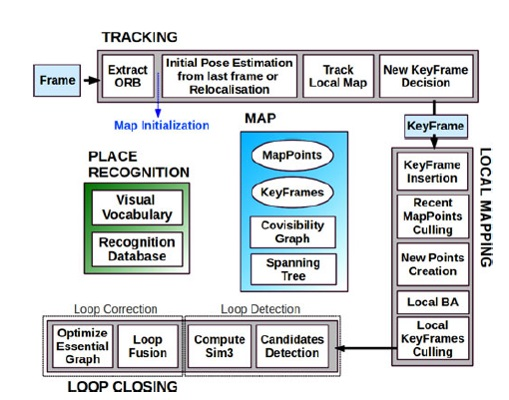
\includegraphics[scale=0.6]{Figure/ORB-SLAM}
\caption{ORB-SLAM system overview}
\end{figure}
  
\end{frame}

\begin{frame}{ORB-SLAM}{Introduction}
  \begin{itemize}
      \item{
      Covisibility graph is an undirected weighted graph. Each node is a keyframe and an edge between two keyframes exists if they share observations of the same map points.
      }
      \item{
      Covisibility graph is too dense and error prone for loop closing operation. An idea of essential graph is proposed in ORB-SLAM method.
      }
      \item{
      Essential graph is a subset of covisibility graph that retains all nodes but less edges, still preserving a strong network that yields accurate results. 
      }
      \item{
      Essential graph contsins spanning trees, subsets of edges from the covisibility graph with high covisibility, and the loop closure edges, resulting in a strong network of cameras.
      }
  \end{itemize}
\end{frame}

\begin{frame}{ORB-SLAM}{Introduction}
    \begin{figure}
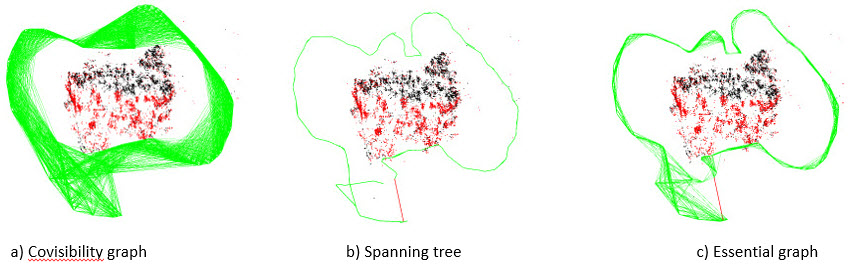
\includegraphics[scale=0.4]{Figure/Graphs}
\caption{Graphs in ORB-SLAM method. a) A covisibility graph. b) A spanning tree. c) An essential graph.}
\end{figure}
  
\end{frame}

\subsection{Tracking thread}
\begin{frame}{ORB-SLAM}{Tracking thread}
  \begin{itemize}
      \item{
      Tracking thread is responsible for the following tasks
      \begin{itemize}
          \item{
          Tracking       
          }
          \item{
          Map initialization
          }
          \item{
          Relocalization when tracking is lost
          }
          \item{
          Track local map
          }
          \item{
          New keyframe decision
          }
      \end{itemize}
      }
      \begin{figure}
          \centering
          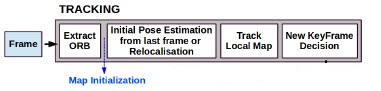
\includegraphics[scale=0.9]{Figure/Tracking}
          \caption{Tracking thread overview}
      \end{figure}
      
  \end{itemize}
\end{frame}

\begin{frame}{ORB-SLAM}{Tracking thread}
    \begin{itemize}
      \item{
      Tracking thread is a process that track a set of points through successive camera frames, and using these tracks to triangulate their 3D position.
      }
      \item{
      Camera pose of each frame is estimated from the relative pose of feature points between the current frame and previous frame.
      }
      \item{
      In ORB-SLAM, tracking thread extracts and uses ORB features from every images in the video sequence.
      }  
    \end{itemize}
\end{frame}
\begin{frame}{ORB-SLAM}{Tracking thread}
\begin{figure}
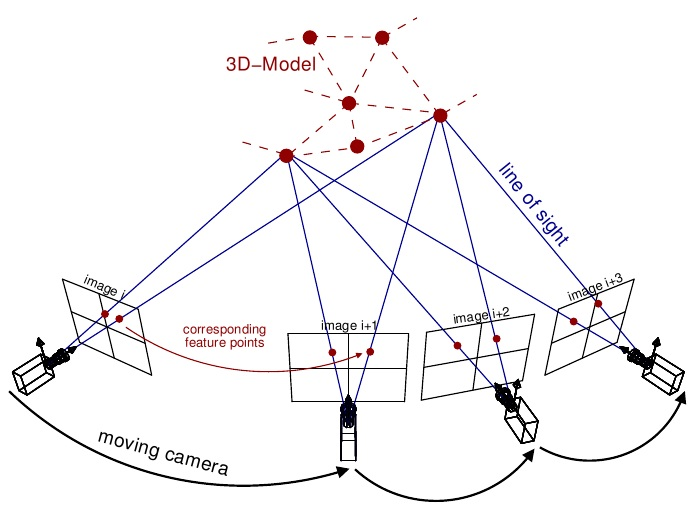
\includegraphics[scale=0.35]{Figure/Triangulation}
\caption{Point triangulation. from http://www.theia-sfm.org/sfm.html}
\end{figure}
    
\end{frame}

\begin{frame}{ORB-SLAM}{Tracking thread: Map initialization}

    \begin{itemize}
    \item{
      Map initialization is the first task of the tracking thread. It triangulates initial 3D correspondences with acceptable accuracy from initial image sequences. 
      }
   \item{
   Matched features $x_{c} \leftrightarrow x_{r}$ between the current frame $f_{c}$ and the reference frame $f_{r}$ are searched to generate initial correspondences.
   }
   \item{
   Reset reference frame if not enough matches are found.
   }
   
    \end{itemize}
\end{frame}

\begin{frame}{ORB-SLAM}{Tracking thread: Map initialization}

    \begin{itemize}
    \item{
   Homography matrix $H_{cr}$ and fundamental matrix $F_{cr}$ are calculated. Tracking thread uses one of these matrices in map initialization process. 
   }
   \item{
   Homography matrix is used if the scene is planar. Fundamental matrix is selected if the scene is nonplanar. 
   }
   \item{
   The map is initialized if the selected matrix passes motion hypotheses tests and gives low reprojection error.
   }
   \item{
      Bundle adjustment is performed to refine initial correspondences and camera poses.
   }
    \end{itemize}
\end{frame}

\begin{frame}{ORB-SLAM}{Tracking thread: Map initialization}
  \begin{figure}
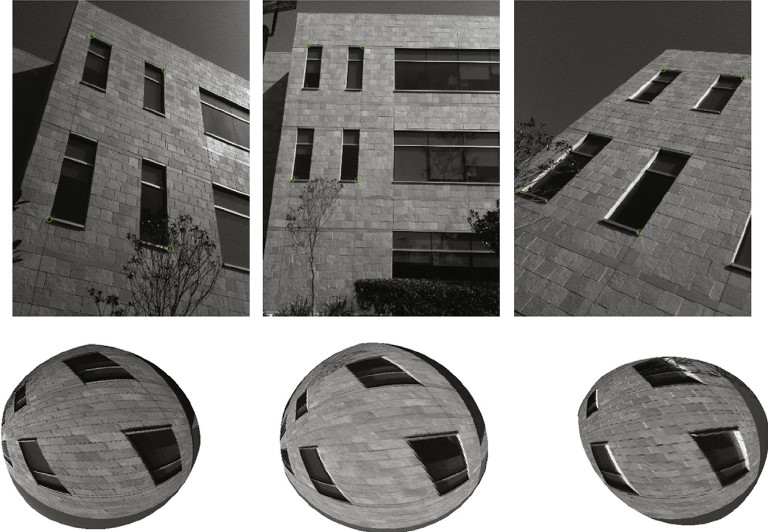
\includegraphics[scale=0.35]{Figure/planar}
\caption{Planar scene. from https://www.researchgate.net/figure/259128816_fig2_Fig-7-Digital-images-of-a-planar-scene-Top-prior-to-projective-frame-registration}
\end{figure}
\end{frame}

\begin{frame}{ORB-SLAM}{Tracking thread: Map initialization}
  \begin{figure}
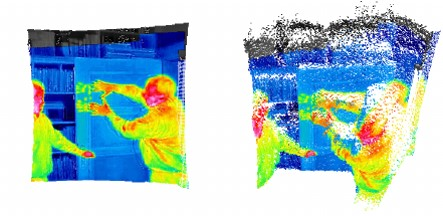
\includegraphics[scale=0.7]{Figure/non_planar}
\caption{Non planar scene. from https://www.researchgate.net/figure/243459165_fig15_Figure-15-Frontal-view-onto-a-non-planar-scene-left-and-a-view-clearly-showing-the}
\end{figure}
\end{frame}

\begin{frame}{ORB-SLAM}{Tracking thread: Tracking}
  \begin{itemize}
      \item{
      Tracking continues the process from map initialization.
      }
      \item{
      If tracking was successful for last frame, camera pose in current frame is predicted with constant velocity motion model.
      }
      \item{
      If not enough matches were found, tracking thread performs wider search of the map points around their position in the last frame.
      }
      \item{
      The pose is optimized with the found correspondences.
      }
  \end{itemize}  
\end{frame}

\begin{frame}{ORB-SLAM}{Tracking thread: Relocalization}
    \begin{itemize}
        \item{
        If tracking is lost, the frame is convert into bag of words and query recognition database for keyframe candidate for global relocalization.
        }
        \item{
        Correspondences with ORB associated to map points in each key frame are computed. RANSAC iterations are performed for each keyframe to find camera pose with $PnP$ algorithm.
        }
        \item{
        If camera pose is found with enough inliers, guided search are performed to find more matches.
        }
        \item{
        The pose is then optimized and tracking procedure continues.
        }
    \end{itemize}    
\end{frame}

\begin{frame}{ORB-SLAM}{Tracking thread: Track local map}
    \begin{itemize}
        \item{
        Once estimated camera pose and an initial set of feature matches are obtained, the map into is projected to the frame and search more map point correspondences.
        }
        \item{
        The local map contains the set of keyframes $K_{1}$, that share map points with the current frame, and a set $K_{2}$ with neighbors to the keyframes $K_{1}$ in the covisibility graph.
        }
        \item{
        Map points seen in $K_{1}$ and $K_{2}$ are searched in the current frame. If found, these map points are added into the current frame and optimized.
        }
    \end{itemize}
\end{frame}

\begin{frame}{ORB-SLAM}{Tracking thread: New keyframe decision}
    \begin{itemize}
        \item{
        The current frame is verified as a keyframe if it meets the conditions
        }
        \item{
        The keyframe decided by the tracking tread is sent to the mapping thread to add into the map.
        }
        \item{
        Keyframes are inserted as fast as possible as it makes the tracking more robust to change in camera movements and rotations.
        }
        \item{
        Redundant keyframes will be culled in the mapping thread.
        }
    \end{itemize}
\end{frame}
\subsection{Mapping thread}
\begin{frame}{ORB-SLAM}{Mapping thread}
    \begin{columns}[T]
\begin{column}{0.8\textwidth}
\begin{itemize}
\item{
Mapping tread is responsible for the following tasks
\begin{itemize}
    \item{
    Keyframe insertion
    }
    \item{
    Map point culling
    }
    \item{
    New map point creation
    }
    \item{
    Local bundle adjustment
    }
    \item{
    Local keyframe culling
    }
\end{itemize}
} 
\end{itemize}
\end{column}
\begin{column}{0.2\textwidth}
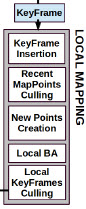
\includegraphics[width=2.5cm]{Figure/localMapping}
\end{column}
\end{columns}
\end{frame}

\begin{frame}{ORB-SLAM}{Mapping thread: Keyframe insertion}
  \begin{itemize}
      \item{
      New keyframes decided by the tracking thread are added into the map.
      }
      \item{
      Nodes and edges in the covisibiilty graph are updated.
      }
      \item{
      Spanning tree and bag of word representation are updated.
      }
  \end{itemize}
\end{frame}

\begin{frame}{ORB-SLAM}{Mapping thread: Map points culling}
  \begin{itemize}
      \item{
      Map points must pass a restrictive test to ensure that they are trackable and not mistakenly triangulated.
      \begin{itemize}
          \item{
          The tracking must find the point in more than the 25 percent of the frames in which it is predicted to be visible.
          }
          \item{
          If more than one keyframe has passed from map point creation, it must be observed from at least three keyframes.
          }
      \end{itemize}
      }
  \end{itemize}
\end{frame}

\begin{frame}{ORB-SLAM}{Mapping thread: New map point creation}
    \begin{itemize}
        \item{
        For each unmatched ORB in an individual frame, unmatched correspondences are searched with other unmatched point in other keyframes.
        }
        \item{
        Newly matched map points are accepted as the new points if they pass the following tests
        \begin{itemize}
            \item{
            Positive depth test in both cameras.
            }
            \item{
            Parallax test.
            }
            \item{
            Reprojection error test.
            }
            \item{
            Scale consistency test.
            }
        \end{itemize}
        }
    \end{itemize}
\end{frame}

\begin{frame}{ORB-SLAM}{Mapping thread: Local bundle adjustment}
  \begin{itemize}
      \item{
      Local BA optimizes the currently processed keyframe ($K_{i}$), all keyframes connected to $K_{i}$ in the covisibility graph ($K_{c}$), and all map points seen by $K_{i}$ and $K_{c}$.
      }
      \item{
      Keyframes that see map points as $K_{i}$ and $K_{c}$ see are included in the optimization but remain fixed.
      }
      \item{
      Outlier are discarded in this process.
      }
  \end{itemize}
\end{frame}

\begin{frame}{ORB-SLAM}{Mapping thread: Keyframe culling}
  \begin{itemize}
      \item{
      As the complexity of bundle adjustment grows with the number of keyframes, deleting redundant keyframes benefits the system in lifelong operation.
      }
      \item{
      Keyframes that has 90 percent similar map points to its three previous keyframes are removed from the map.
      }
  \end{itemize}
\end{frame}

\subsection{Loop closing thread}
\begin{frame}{ORB-SLAM}{Loop closing}
  \begin{itemize}
      \item{
      Loop closing takes the last keyframe processed by the mapping thread to detect and close the loop.
      }
      \item{
      Loop closing performs the following tasks
      \begin{itemize}
          \item{
          Loop candidates detection.
          }
          \item{
          Similarity transformation estimation.
          }
          \item{
          Loop fusion.
          }
          \item{
          Essential graph optimization.
          }
      \end{itemize}
      }
  \end{itemize}
  \begin{figure}
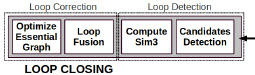
\includegraphics[scale=0.7]{Figure/LoopClosing}
\caption{Loop closing overview.}
\end{figure}
\end{frame}

\begin{frame}{ORB-SLAM}{Loop closing thread: Loop candidates detection}
  \begin{itemize}
      \item{
      Similarity score is computed between the bag of word vector of the last keyframe $K_{i}$ with all of its neighbors in the covisibility graph. The lowest score $s_{min}$ is obtained.
      }
      \item{
      Recognition database is queried, keyframe whose score is lower than $s_{min}$ are not considered as loop candidates.
      }
      \item{
      All keyframes whose are directly connected to $K_{i}$ are also not considered as loop candidates.
      }
  \end{itemize}
\end{frame}

\begin{frame}{ORB-SLAM}{Loop closing thread: Similarity transformation estimation}
  \begin{itemize}
      \item{
      ORB-associated correspondences between the current keyframe and the loop candidate keyframes are calculated.
      }
      \item{
      RANSAC iterations are performed with each candidate to find a similarity transformation. 
      }
      \item{
      If the similarity is found with enough inliers, the transformation is optimized and more correspondences are searched.
      }
      \item{
      After adding more correspondences, the transformation is optimized again. If the transformation is supported by enough inliers, that loop candidate is accepted.
      }
  \end{itemize}
\end{frame}

\begin{frame}{ORB-SLAM}{Loop closing thread: Loop fusion}
  \begin{itemize}
      \item{
      Once loop closing is detected and verified, two keyframes are merged together.
      }
      \item{
      The correction for this action must be done and propagated to their neighbor keyframes in covisibility graph so they can update their proterties(i.e. recalculate transformation matrix, concatenated edges in covisibility graph). 

      }
  \end{itemize}
\end{frame}

\begin{frame}{ORB-SLAM}{Loop closing thread: Essential graph optimization}
  \begin{itemize}
      \item{
      Pose graph optimization over the Essential graph is performed to effectively close the loop.
      }
      \item{
      Scale drift is corrected, each map point is transformed according to the correction.
      }
  \end{itemize}
  
  \begin{figure}
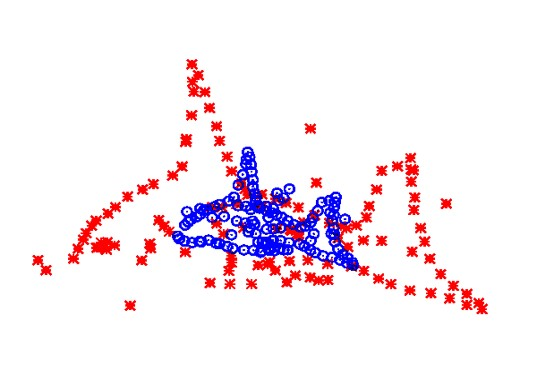
\includegraphics[scale=0.3]{Figure/scaleDrift}
\caption{Scale drift.}
\end{figure}
  
\end{frame}


\subsection{ORB-SLAM example}
\begin{frame}{ORB-SLAM}{Example}
  \begin{figure}
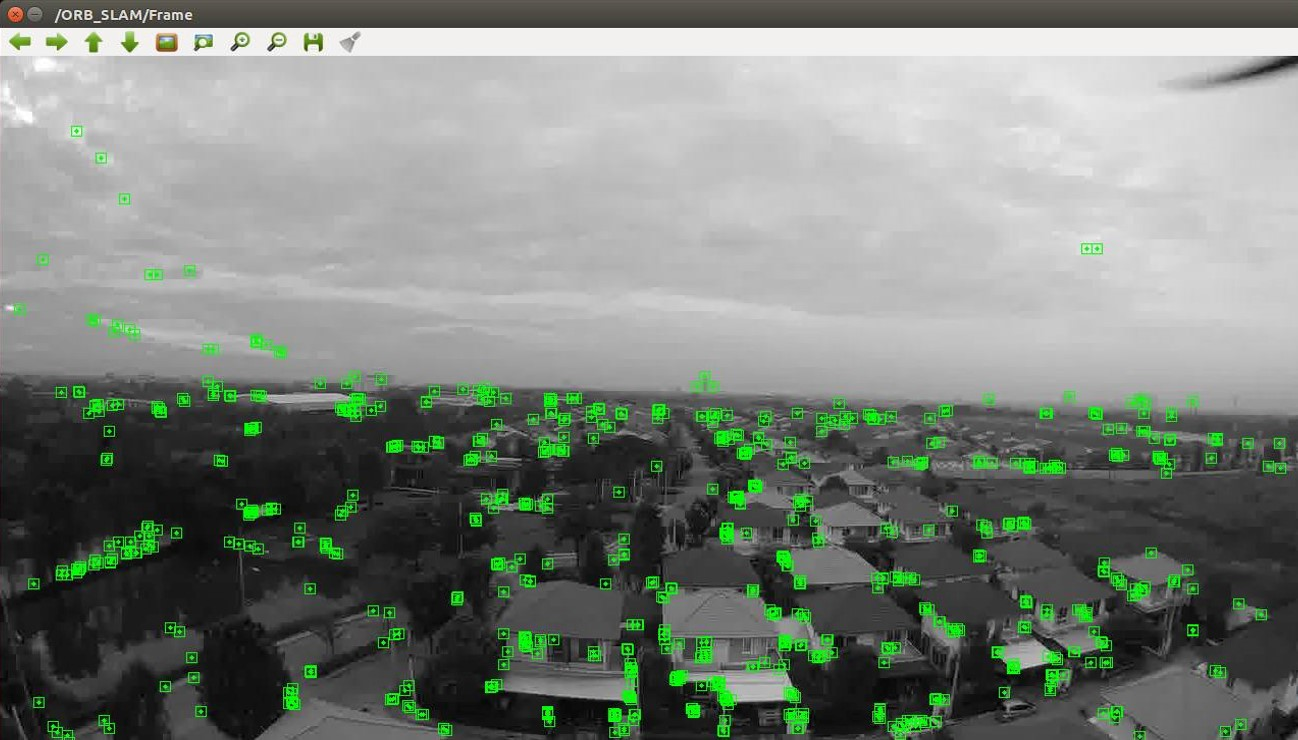
\includegraphics[scale=0.3]{Figure/ORBtrack}
\caption{ORB-SLAM example: tracking.}
\end{figure}
\end{frame}

\begin{frame}{ORB-SLAM}{Example}
  \begin{figure}
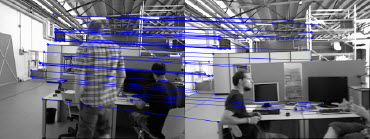
\includegraphics[scale=0.9]{Figure/ORBexMapping}
\caption{ORB-SLAM example: mapping.}
\end{figure}
\end{frame}

\begin{frame}{ORB-SLAM}{Example}
  \begin{figure}
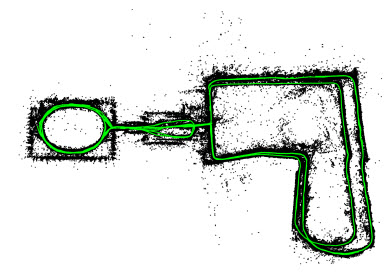
\includegraphics[scale=0.7]{Figure/ORBexLoopClosing}
\caption{ORB-SLAM example: loop closing.}
\end{figure}
\end{frame}



\end{document}


